\documentclass[11pt,a4paper]{article}

\usepackage[margin=1in]{geometry}
\usepackage{graphicx}
\usepackage{booktabs}
\usepackage{array}
\usepackage{longtable}
\usepackage{hyperref}
\usepackage{xcolor}
\usepackage{enumitem}
\usepackage{amsmath}
\usepackage{float}
\usepackage{listings}

\hypersetup{
  colorlinks=true,
  linkcolor=blue,
  urlcolor=blue,
  citecolor=blue
}

\lstset{
  basicstyle=\ttfamily\small,
  breaklines=true,
  frame=single,
  columns=fullflexible
}

\title{\textbf{Parallel Travelling Salesman Problem Solver}\\
\large Island-Model Genetic Algorithm with MPI}
\author{Parallel Programming Project}
\date{June 2026}

\begin{document}
\maketitle

\begin{abstract}
This report describes a parallel solver for the Travelling Salesman Problem
(TSP). The implementation uses an island-model Genetic Algorithm (GA) written in
C++ and parallelized with MPI. Each MPI process is an independent island that
evolves a population of tours. At fixed synchronization intervals, all islands
cooperate by finding the global best tour with \texttt{MPI\_Allreduce} and
broadcasting the owner tour with \texttt{MPI\_Bcast}. Other islands do not clone
the whole tour; instead, they splice random contiguous segments of the global
best into their own population through order crossover. This keeps the search
diverse while still spreading useful sub-routes.

The repository also contains Python tools for visualization, validation, and
plot generation. The Python code does not implement the TSP algorithm; it only
drives the C++ executable or reads output files generated by the solver. The
experimental results cover correctness validation, input-size selection,
granularity/load balance, and speedup with and without communication time.
\end{abstract}

\tableofcontents
\newpage

\section{Project Overview}

\subsection{Problem Statement}
Given a set of $N$ cities with two-dimensional coordinates, the Travelling
Salesman Problem asks for a closed tour that visits every city exactly once and
returns to the starting city while minimizing total Euclidean distance. For a
tour $T = (t_0, t_1, \ldots, t_{N-1})$, the objective value is:

\[
  L(T) = \sum_{i=0}^{N-1} d(t_i, t_{(i+1) \bmod N})
\]

where $d(a,b)$ is the Euclidean distance between city $a$ and city $b$.
TSP is NP-hard, so the project uses a heuristic search method instead of exact
enumeration for large instances.

\subsection{Repository Structure}
The project is organized as follows:

\begin{itemize}[leftmargin=*]
  \item \texttt{cpp/}: C++ implementation of the GA, local search, MPI solver,
  sequential baseline, and unit tests.
  \item \texttt{python/}: plotting, visualization, validation, and experiment
  orchestration tools.
  \item \texttt{data/}: city-coordinate input files and a generator.
  \item \texttt{cluster/}: OpenMPI installation, SSH setup, synchronization, and
  cluster launch scripts.
  \item \texttt{results/}: CSV files and figures produced by the experiments.
  \item \texttt{report/}: report and presentation materials.
\end{itemize}

\subsection{Main Source Files}
The full solver is in C++:

\begin{itemize}[leftmargin=*]
  \item \texttt{cpp/ga\_core.hpp}: reads city files, builds the distance matrix,
  evaluates tours, creates random tours, performs tournament selection, order
  crossover (OX), mutation, and one generation of evolution.
  \item \texttt{cpp/local\_search.hpp}: implements 2-opt, Or-opt, and
  \texttt{polish()} for optional memetic local improvement.
  \item \texttt{cpp/tsp\_island.cpp}: main MPI island-model solver.
  \item \texttt{cpp/tsp\_sequential.cpp}: single-process baseline.
  \item \texttt{cpp/test\_ga\_core.cpp} and \texttt{cpp/test\_local\_search.cpp}:
  unit tests for genetic operators and local search.
\end{itemize}

\section{Sequential Genetic Algorithm}

\subsection{Representation}
Each individual is a permutation of city indices. For example, for $N=5$, a
tour may be:

\begin{center}
\texttt{[2, 0, 4, 1, 3]}
\end{center}

The tour is closed implicitly, so the last city connects back to the first city.
This representation guarantees that a valid individual can be evaluated directly
as a TSP route.

\subsection{Fitness Evaluation}
The solver precomputes a flat $N \times N$ Euclidean distance matrix. The
fitness value is the total tour length. Smaller values are better.

\subsection{Selection, Crossover, and Mutation}
The GA uses:

\begin{itemize}[leftmargin=*]
  \item Tournament selection with tournament size $k=5$.
  \item Order crossover (OX), which copies a contiguous segment from one parent
  and fills the remaining positions using the order of the second parent.
  \item Mutation by swapping two cities and reversing one random segment.
  \item Elitism of one best individual per generation.
\end{itemize}

\subsection{Local Search}
The optional memetic extension applies local search to the best individual every
\texttt{--twoopt} generations. The local improvement consists of:

\begin{itemize}[leftmargin=*]
  \item 2-opt: remove two crossing edges and reconnect the tour by reversing a
  segment.
  \item Or-opt: move a short contiguous segment to a better insertion position.
\end{itemize}

\section{Parallelization Design}

\subsection{Parallelism Level}
The implementation uses coarse-grained task-level parallelism. Each MPI process
owns a complete GA population and performs an independent stochastic search.
The city data and distance matrix are replicated on every process.

The design also has an exploratory-search characteristic: different islands
explore different regions of the search space due to different random seeds.
Therefore, the decomposition is best described as a hybrid of task decomposition
and exploratory decomposition.

\subsection{Decomposition Technique}
The selected decomposition is \textbf{exploratory decomposition with replicated
input data}. Each island receives the same TSP instance but evolves a different
population. This is suitable for a heuristic optimization problem because the
main work is search, not deterministic matrix processing.

The alternatives were less suitable:

\begin{itemize}[leftmargin=*]
  \item Pure data decomposition is not natural because a single tour depends on
  the global order of all cities.
  \item Recursive decomposition is more appropriate for divide-and-conquer exact
  search, not for the selected GA.
  \item Speculative decomposition is possible for exact branch-and-bound but was
  not the focus of this project.
\end{itemize}

\subsection{Mapping Technique}
The mapping is a one-dimensional process-to-island assignment:

\[
  \text{rank } r \longrightarrow \text{island } r
\]

Each rank stores:

\begin{itemize}[leftmargin=*]
  \item one local population of tours,
  \item one local vector of tour lengths,
  \item one local pseudo-random generator with seed \texttt{base + rank * 1000},
  \item the replicated city coordinates and distance matrix.
\end{itemize}

For the cluster experiment, the hostfile uses a sequential round-robin list of
hosts. This spreads ranks across four machines and supports up to 48 ranks, with
12 ranks per machine as the common physical-core limit.

\subsection{Communication Strategy}
Communication is periodic and collective. Every \texttt{--sync} generations:

\begin{enumerate}[leftmargin=*]
  \item Each rank finds its local best individual.
  \item \texttt{MPI\_Allreduce} with \texttt{MPI\_MINLOC} finds the globally best
  length and the owner rank.
  \item The owner rank broadcasts the best tour using \texttt{MPI\_Bcast}.
  \item Non-owner ranks perform partial migration by combining a segment of the
  global best with local individuals.
\end{enumerate}

This is a blocking collective communication strategy. The logical topology is
global collective communication rather than a ring or master-slave topology.
There is no permanent master rank during evolution; all ranks participate
symmetrically. Rank 0 is used only for final reporting and file output.

\subsection{Migration Policy}
A naive island GA can broadcast the full best individual and clone it into every
island. That is fast but dangerous: diversity collapses and all islands may
converge to the same local optimum.

This implementation uses partial global-best migration:

\begin{itemize}[leftmargin=*]
  \item The global best tour is broadcast to all islands.
  \item Each non-owner island selects several worst individuals.
  \item For each replacement, it uses OX crossover between the global best and a
  random local mate.
  \item The child replaces one of the worst local individuals.
\end{itemize}

Only sub-routes are shared. Random cut points and local mates keep the resulting
population different on each island.

\subsection{Load Balancing Considerations}
In the default mode, every rank uses the same population size, so compute work is
approximately balanced. This is appropriate for machines with similar effective
capacity or for a controlled experiment where ranks per machine are limited by
the slowest machine.

The solver also contains an optional \texttt{--auto-balance} mode. It performs a
small local benchmark on each process, gathers the measured times, and assigns a
larger population to faster ranks. The allocation is clamped between 0.5x and 2x
of the original population to avoid unstable decisions from noisy measurements.

\subsection{Early Stopping}
If \texttt{--patience} is enabled, the solver stops when the global best does not
improve for a fixed number of generations. Because the same global best value is
known to all ranks after each synchronization, every rank can make the same stop
decision without an extra control message.

\section{Parallel Algorithm Pseudocode}

\begin{lstlisting}[language={},caption={Island-model GA with partial global-best migration}]
Input: city file, generations G, population size P,
       sync interval S, migrants M

MPI_Init()
rank <- MPI_Comm_rank()
size <- MPI_Comm_size()

coords <- read_cities(file)
D <- distance_matrix(coords)
rng <- seed + rank * 1000

pop <- P random tours
len <- evaluate all tours

for g = 1 to G:
    evolve_one_generation(pop, len, D)

    if twoopt enabled and g % twoopt == 0:
        polish local best with 2-opt and Or-opt

    if S > 0 and size > 1 and g % S == 0:
        local_best <- best tour on this rank
        (global_value, owner) <- MPI_Allreduce(MINLOC, local_best)

        if rank == owner:
            buffer <- local_best_tour
        MPI_Bcast(buffer, owner)

        if rank != owner:
            repeat M times:
                worst <- worst local individual
                mate <- random local individual
                child <- OX(buffer, mate)
                replace worst by child

        update convergence-stop state
        if stalled for patience generations:
            break

final_local_best <- best tour on this rank
(global_best, owner) <- MPI_Allreduce(MINLOC, final_local_best)
owner sends best tour to rank 0 if needed
rank 0 writes route, history, stats
MPI_Finalize()
\end{lstlisting}

\section{Implementation and Instrumentation}

\subsection{Command-Line Interface}
The main solver accepts the following key arguments:

\begin{itemize}[leftmargin=*]
  \item \texttt{--gens}: maximum number of generations.
  \item \texttt{--pop}: population size per island.
  \item \texttt{--sync}: migration interval; \texttt{0} disables sharing.
  \item \texttt{--migrants}: number of individuals recombined with the global
  best per synchronization.
  \item \texttt{--patience}: convergence-stop patience.
  \item \texttt{--twoopt}: local-search period.
  \item \texttt{--out}: output tour and convergence history.
  \item \texttt{--stats}: per-rank CSV statistics.
  \item \texttt{--live}: JSONL stream for live visualization.
\end{itemize}

\subsection{Timing Metrics}
The solver separates communication time from total elapsed time:

\begin{itemize}[leftmargin=*]
  \item \texttt{comm\_s}: time spent inside MPI communication calls.
  \item \texttt{total\_s}: wall-clock elapsed time on a rank.
  \item \texttt{compute\_s}: estimated as \texttt{total\_s - comm\_s}.
  \item \texttt{makespan\_s}: maximum total time over all ranks.
\end{itemize}

These metrics are written to the \texttt{--stats} CSV file and used by
\texttt{python/experiments.py} to draw the required result figures.

\subsection{Cluster Environment}
The cluster setup uses four machines and up to 48 MPI ranks. OpenMPI 5.0.9 is
source-built and pinned at \texttt{/opt/openmpi-5.0.9} on all nodes to avoid
runtime incompatibilities. The launch script uses:

\begin{itemize}[leftmargin=*]
  \item \texttt{--map-by seq}: sequential mapping from the hostfile.
  \item \texttt{--bind-to none}: avoids topology-dependent binding problems on
  heterogeneous machines.
  \item a pinned \texttt{prted} launch agent path for remote nodes.
\end{itemize}

\section{Correctness Validation}

\subsection{Permutation Validity}
The solver represents a route as a permutation of city IDs. The unit tests check
that crossover and mutation preserve valid permutations. The validation script
\texttt{python/validate\_tour.py} independently verifies that a produced route:

\begin{enumerate}[leftmargin=*]
  \item has exactly $N$ city indices,
  \item contains every city from $0$ to $N-1$ exactly once,
  \item has a recomputed length matching the reported best length.
\end{enumerate}

\subsection{Small-Instance Exact Check}
For $N \le 10$, the validation script can brute-force all tours with city 0 fixed
as the first city. This gives the true optimum and allows the GA result to be
checked against the exact solution. The repository includes validation logs for
small and larger instances in \texttt{results/}.

\subsection{Parallel Communication Check}
The per-rank history files show that migration changes the behavior of non-owner
islands after synchronization points. In one cluster run, rank 2 held the best
tour before synchronization at generation 20. After the synchronization, weaker
islands moved toward that better solution, but did not become identical. This
matches the intended partial-migration behavior: useful route segments spread,
while population diversity is preserved.

\section{Experimental Results}

\subsection{Experiment 1: Input Size Selection}
The requirement asks for an input-size experiment using the number of processes
equal to the number of physical CPU cores. The cluster configuration uses up to
48 ranks. The runtime is measured in two cases: total time including
communication, and estimated compute time excluding communication.

The first sweep used a fixed 400-generation run to understand the growth trend.
It showed that larger instances increase compute work and communication volume,
but the run was still too short for the required 2--3 minute target.

\begin{table}[H]
\centering
\caption{Runtime versus input size with 48 MPI ranks}
\begin{tabular}{rrrr}
\toprule
$N$ & Total time (s) & Communication (s) & Compute only (s) \\
\midrule
100  & 1.2427 & 1.1512 & 0.0915 \\
200  & 1.0223 & 0.8770 & 0.1453 \\
400  & 1.7410 & 1.4027 & 0.3383 \\
800  & 2.9824 & 1.9272 & 1.0552 \\
1200 & 4.2491 & 2.4806 & 1.7685 \\
2400 & 8.1918 & 3.8092 & 4.3826 \\
\bottomrule
\end{tabular}
\end{table}

\begin{figure}[H]
\centering
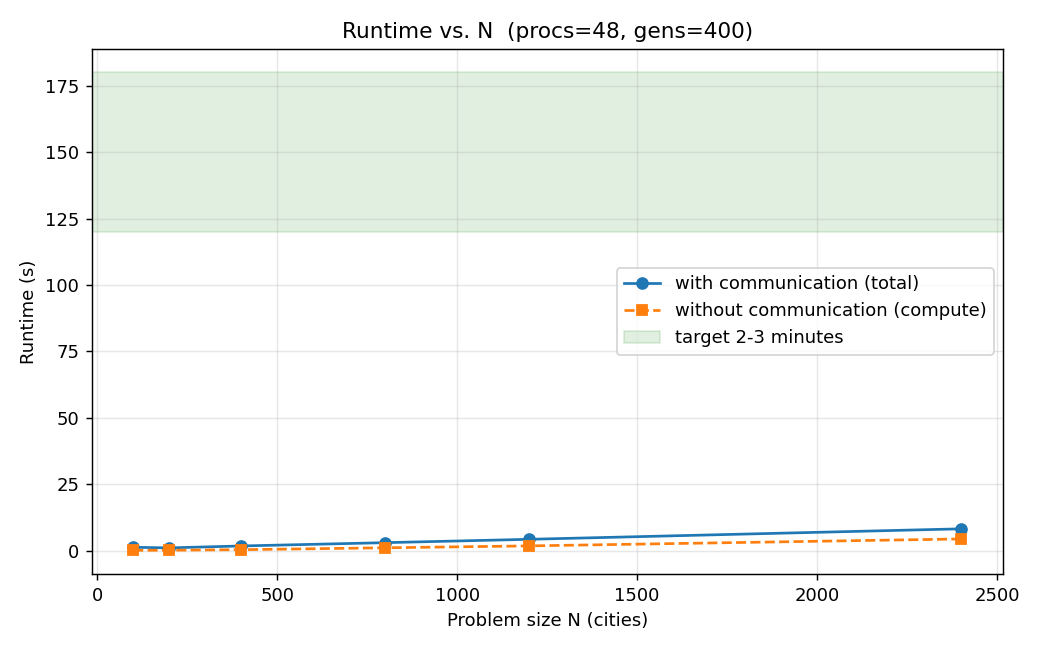
\includegraphics[width=0.85\linewidth]{../results/exp_size.png}
\caption{Initial runtime sweep versus number of cities, with and without communication time.}
\end{figure}

To satisfy the 2--3 minute requirement, the final selection fixed
\texttt{procs=48}, \texttt{sync=20}, and increased the generation count to
\texttt{gens=10500}. The clean selection run is:

\begin{table}[H]
\centering
\caption{Final $N^*$ selection at 48 ranks, 10500 generations}
\begin{tabular}{rrrr}
\toprule
$N$ & Total time (s) & Communication (s) & Compute only (s) \\
\midrule
1200 & 54.54  & 25.90 & 28.65 \\
1800 & 86.99  & 34.33 & 52.66 \\
2400 & 154.27 & 64.05 & 90.22 \\
\bottomrule
\end{tabular}
\end{table}

The selected input size is therefore:

\begin{center}
\fbox{\textbf{$N^* = 2400$ cities, \texttt{gens* = 10500}, 48 ranks}}
\end{center}

The official repeated run stored in \texttt{results/nstar\_run.log} reports a
makespan of \textbf{145.97 seconds}, which lies inside the required 120--180
second interval. Other repeated measurements at the same configuration were
159.14s and 154.27s, also inside the target range.

\subsection{Experiment 2: Granularity and Load Balance}
For the granularity experiment, the program is run with the selected input size
$N^*=2400$, \texttt{gens=10500}, and 48 ranks. Each rank is one island, so the
granularity is one GA population per process. The required stacked bar chart
shows compute time and communication time in the same column for each process.

\begin{figure}[H]
\centering
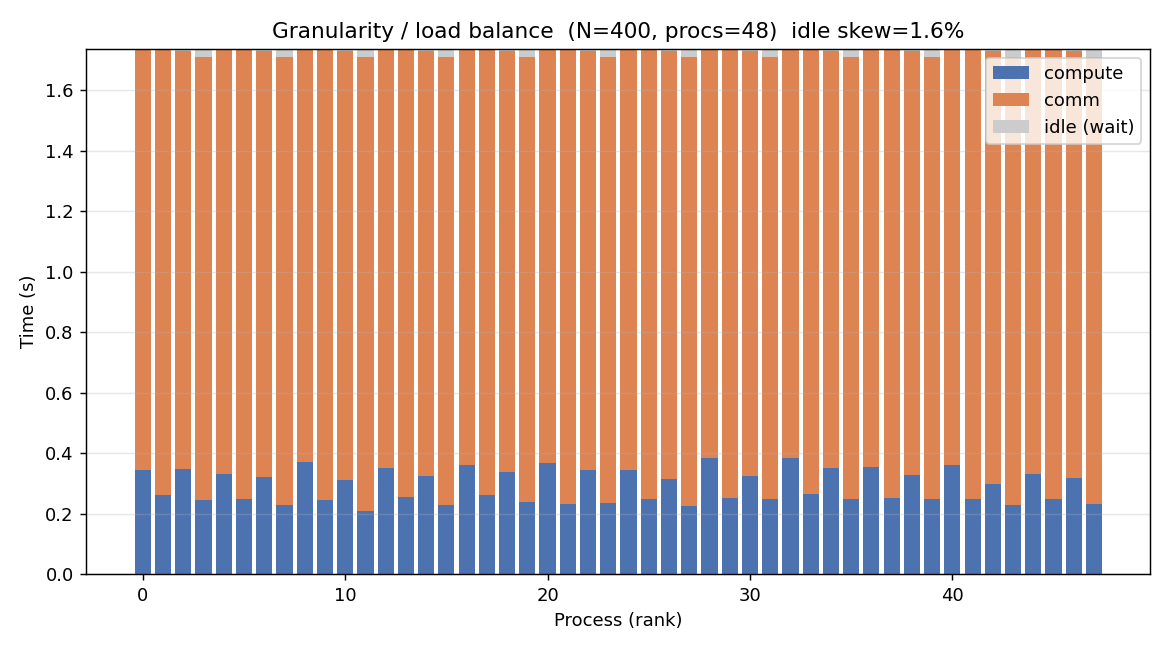
\includegraphics[width=0.9\linewidth]{../results/exp_gran.png}
\caption{Per-rank compute and communication time for the granularity experiment.}
\end{figure}

The measured idle skew is about 1.8\%, which is below the 25\% imbalance
threshold. Therefore, the system is considered load-balanced for this run. The
main difference between ranks is not idle waiting but the split between compute
and communication time, which is expected when ranks synchronize through
blocking MPI collectives.

\subsection{Experiment 3: Speedup}
The speedup experiment uses a fixed total workload and varies the number of
processes. Following the requirement, this experiment uses $2N^* = 4800$ cities
with \texttt{gens=400}, \texttt{sync=20}, and a fixed total population of 480
individuals split over the active ranks. The measured values are:

\begin{table}[H]
\centering
\caption{Speedup experiment}
\begin{tabular}{rrrrrrr}
\toprule
Procs & Total (s) & Comm (s) & Compute (s) & Speedup & No-comm speedup & Eff. \\
\midrule
1  & 16.3636 & 0.0000 & 16.3636 & 1.0000 & 1.0000  & 1.0000 \\
2  & 9.6910  & 3.6071 & 6.0840  & 1.6885 & 2.6896  & 0.8443 \\
4  & 4.7995  & 2.1130 & 2.6865  & 3.4094 & 6.0910  & 0.8524 \\
8  & 3.3492  & 1.9690 & 1.3802  & 4.8858 & 11.8559 & 0.6107 \\
16 & 2.8577  & 2.0346 & 0.8231  & 5.7261 & 19.8806 & 0.3579 \\
32 & 3.6413  & 2.6965 & 0.9448  & 4.4939 & 17.3200 & 0.1404 \\
48 & 4.0388  & 2.8897 & 1.1491  & 4.0516 & 14.2398 & 0.0844 \\
\bottomrule
\end{tabular}
\end{table}

\begin{figure}[H]
\centering
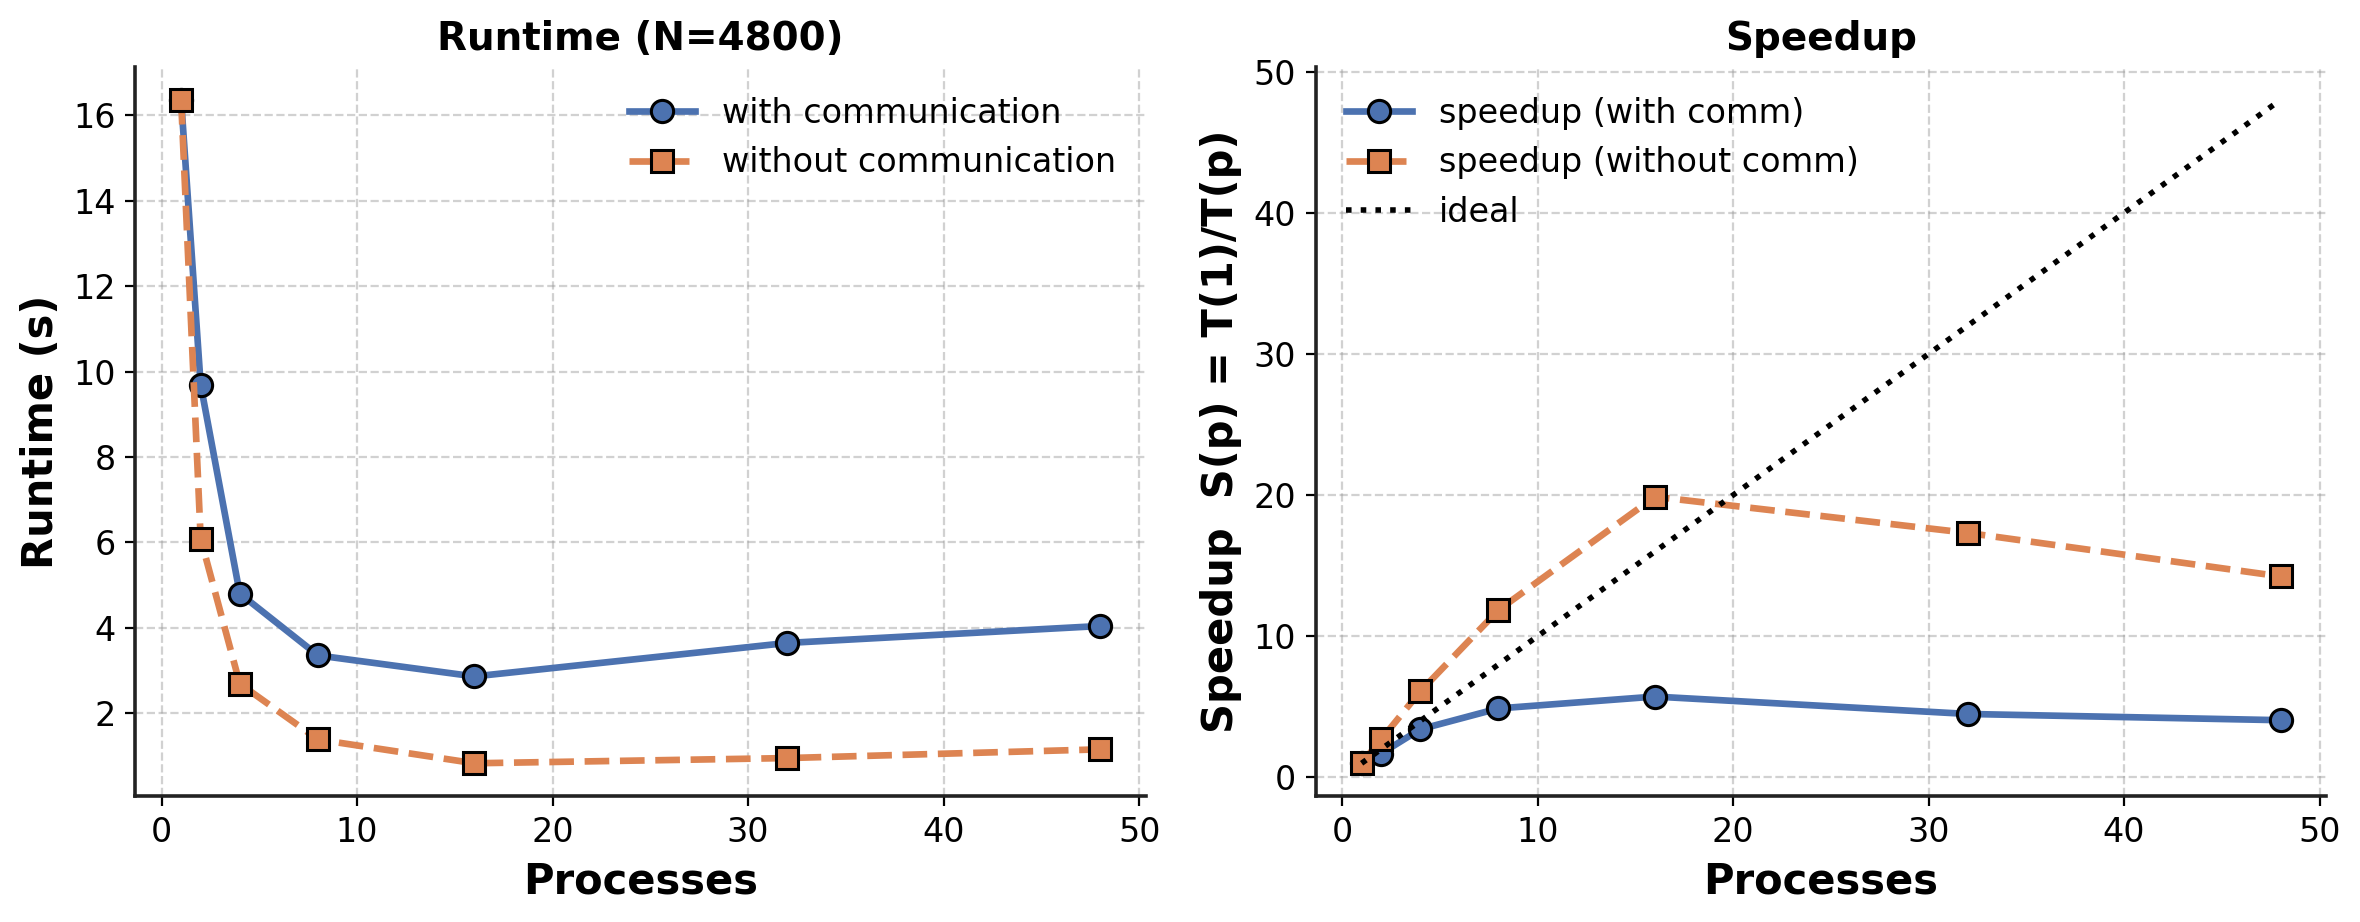
\includegraphics[width=0.9\linewidth]{../results/exp_speedup.png}
\caption{Runtime and speedup as the number of processes changes.}
\end{figure}

The speedup improves up to 16 processes and then decreases. This means the
parallel computation scales initially, but the communication and synchronization
overhead becomes dominant at high process counts. The no-communication speedup
is much higher, showing that the GA computation itself is parallelizable. The
limiting factor is the cost of repeated collective communication on the real
cluster network.

\section{Discussion}

\subsection{Why the Island Model Fits TSP}
The island model is a natural fit for TSP because the problem is a global
combinatorial search. Multiple populations can explore different areas of the
solution space without requiring communication at every generation. This reduces
the cost compared with fine-grained parallel GA designs.

\subsection{Communication Trade-Off}
The \texttt{--sync} parameter controls the trade-off between cooperation and
overhead. A small interval spreads good information quickly but increases
communication cost and can reduce diversity. A large interval reduces overhead
but makes the islands behave more like independent runs. The no-sharing mode
\texttt{--sync 0} is useful as a baseline.

\subsection{Granularity}
The chosen granularity is coarse: one full GA population per process. This
reduces communication frequency and makes the program easier to run on a
heterogeneous cluster. The drawback is that very small TSP instances do not have
enough computation per process, so communication dominates.

\subsection{Limitations}
The current implementation is a heuristic solver. It does not guarantee the
global optimum for large TSP instances. The exact check is only feasible for
small $N$. The selected $N^*=2400$ configuration satisfies the 2--3 minute
runtime target, but the result is still affected by normal run-to-run variation
on a heterogeneous laptop cluster.

\section{Conclusion}
This project implements a complete MPI-based parallel TSP solver using an
island-model Genetic Algorithm. The parallelism is coarse-grained and
task/exploratory in nature. Each MPI rank owns an island and communicates only
periodically through blocking MPI collectives. The mapping is one-dimensional:
rank to island. The communication topology is global collective communication
using \texttt{MPI\_Allreduce} and \texttt{MPI\_Bcast}.

Correctness is checked through permutation tests, independent route-length
validation, and brute-force validation for small instances. The experimental
results show balanced work distribution and meaningful speedup up to a moderate
number of processes. At high process counts, communication overhead dominates,
which is visible in the difference between total speedup and no-communication
speedup.

\section*{Appendix: Reproducible Commands}

\begin{lstlisting}[language=bash]
# Build
cd cpp
make
make test

# Local MPI run
mpirun --oversubscribe -np 4 ./cpp/tsp_island \
  data/cities_50.txt --gens 500 --sync 20

# Cluster run
bash cluster/run_cluster.sh cluster/hosts.seq48 48 \
  ./cpp/tsp_island data/cities_400.txt \
  --gens 400 --sync 20 --stats results/run.csv

# Required experiment figures
python3 python/experiments.py size \
  --procs 48 --sizes 100 200 400 800 1200 2400

python3 python/experiments.py gran \
  --procs 48 --size 400

python3 python/experiments.py speedup \
  --procs 1 2 4 8 16 32 48 --size 400
\end{lstlisting}

\end{document}
